\documentclass[11pt]{article}
\usepackage{amsmath, amssymb, amsthm}
\usepackage[retainorgcmds]{IEEEtrantools}
\usepackage{esint}

\usepackage[pdftex]{graphicx}

\usepackage{marginnote}

\usepackage{fancyhdr}

%Format stuff
\pagestyle{fancy}
\headheight 35pt

%Header info
\chead{\Large \textbf{Vector Field Theory}}
\lhead{}
\rhead{}

\begin{document}
\section{Green's Theorem}
	Green's Theorem is defined for unions of \textbf{simple} regions - that is, the boundary of $D$ bounded by a curve $\gamma$ is crossed at most twice by a line parallel to an axis. When there are multiple boundaries, trace them so that $D$ is always to the left.
	
	If the curve $\gamma$ traced in the clockwise direction is denoted $\gamma -$, then
	\begin{equation}
		\int_{\gamma -} \vec{F} \cdot d\vec{x} = - \int_\gamma \vec{F} \cdot d\vec{x}
	\end{equation}
	
	\subparagraph{Green's Theorem} Let \marginnote{Green's Theorem?}$D$ be a bounded plane that is a union of simple regions, each with a boundary consisting of a piecewise smooth curve. Let $F$ and $G$ be continuously differentiable real-vaued functions on $D$ and $\gamma$. Then
	\begin{equation}
		\int_D \left( \frac{\partial G}{\partial x} - \frac{\partial F}{\partial y} \right) dxdy = \ointctrclockwise_\gamma F\ dx + G\ dy
	\end{equation}
	
	\subparagraph{Changing Paths}
		Given a region between two closed curves $\gamma$ and $\delta$ that are traced in the same direction,
		\begin{equation}
			\frac{\partial G}{\partial x} - \frac{\partial F}{\partial y} = 0 \rightarrow \int_\gamma F\ dx + G\ dy = \int_\delta F\ dx + G\ dy
		\end{equation}
		
	\subparagraph{Path Independence Principle} If \marginnote{Path independence?}a plane vector field $\vec{F}(x, y) = ( F(x, y), G(x, y) )$ satisfies $\partial G / \partial x - \partial F / \partial y = 0$ in a region whose boundary is the union of two paths $\gamma_1$ and $\gamma_2$ with common start and end points, then
		\begin{equation}
			\int_{\gamma_1} \vec{F} \cdot d\vec{x} = \int_{\gamma_2} \vec{F} \cdot d\vec{x}
		\end{equation}
		
	\subparagraph{Physical Interpretations} If \marginnote{Unit tangent and normal vectors?}$\gamma$ has a smooth parametrization $g(t) = (g_1(t), g_2(t))$, $a \leq t \leq b$, and has a nonzero derivative, then the unit tangent and normal vectors (Figure \ref{fig:greens})  are
		\begin{equation}
			\vec{t}(t) = \frac{g'(t)}{|g'(t)|} = (\left( \frac{g'_1(t)}{|g'(t)|}, \frac{g'_2(t)}{|g'(t)|} \right)
		\end{equation}
		
		\begin{equation}
			\vec{n}(t) = \left( \frac{g'_2(t)}{|g'(t)|}, \frac{-g'_1(t)}{|g'(t)|} \right)
		\end{equation}
		
		\begin{figure}[htb]
			\centering
			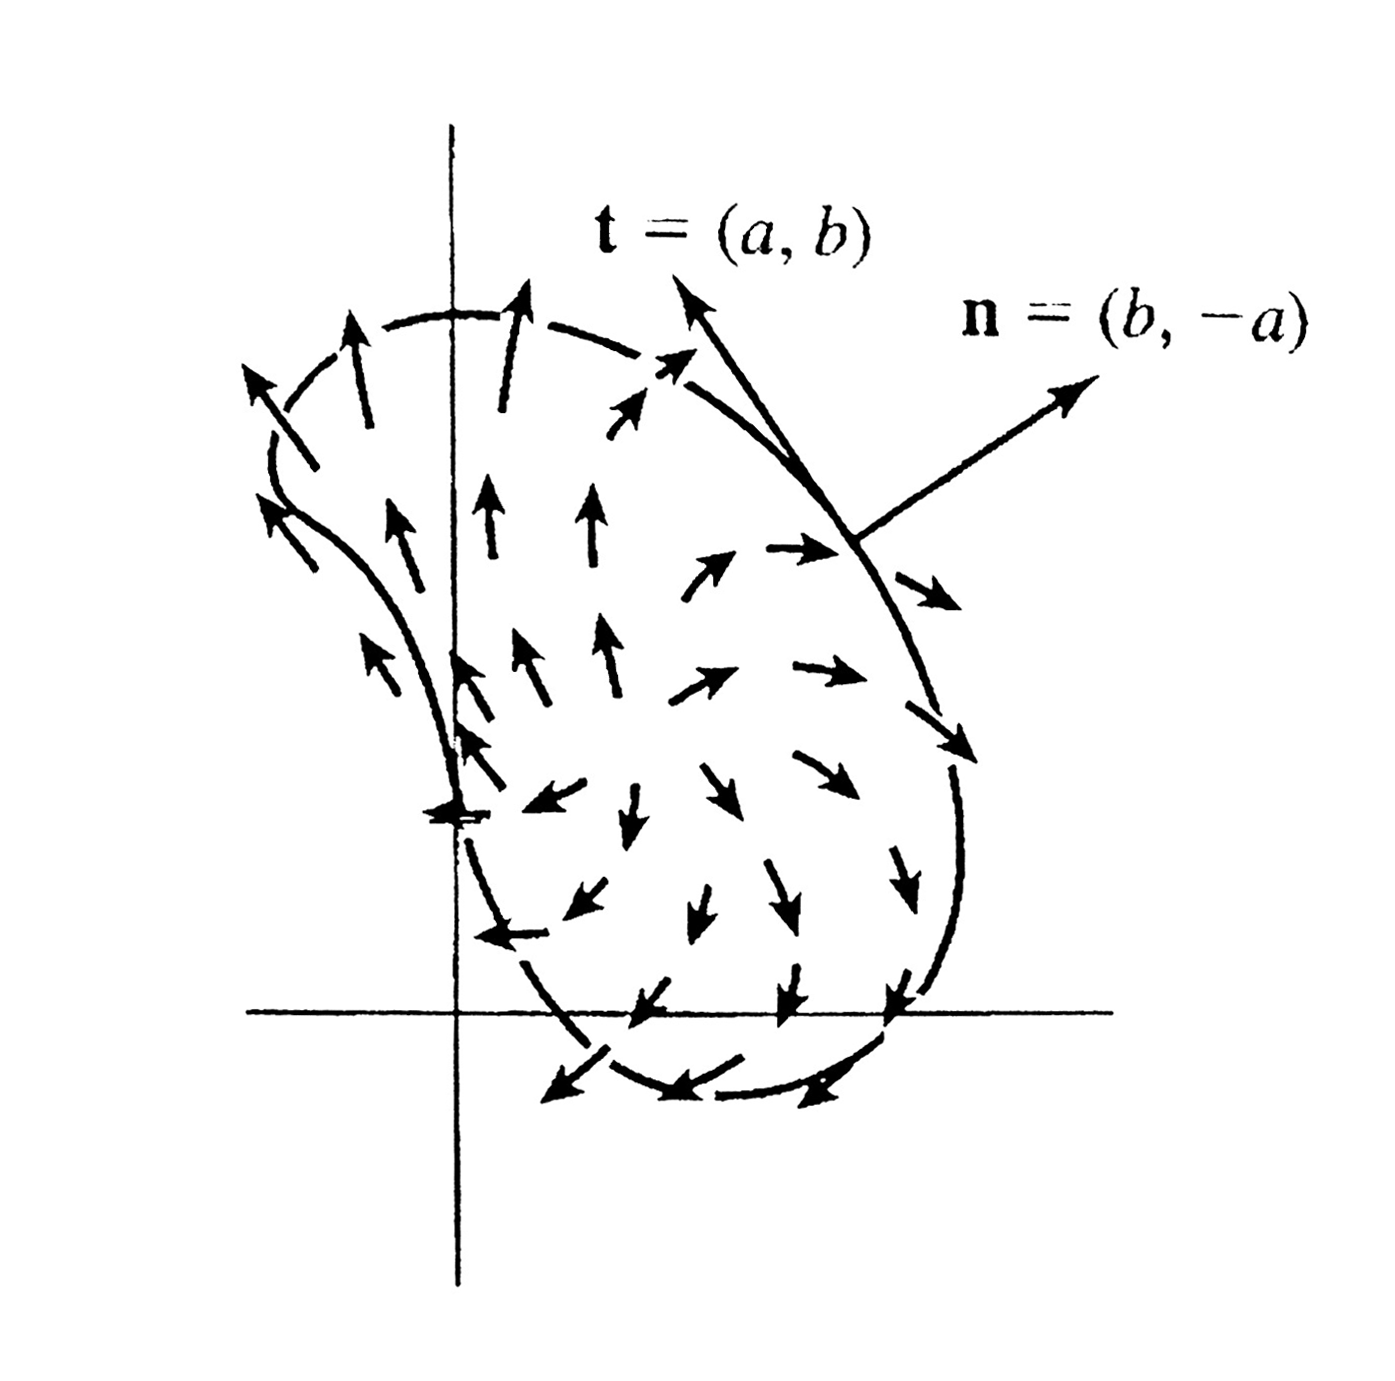
\includegraphics[width=0.4\textwidth]{greens.png}
			\caption{Tangent and normal vectors of $\gamma$}
			\label{fig:greens}
		\end{figure}
		
	\subparagraph{Stokes's Theorem in the Plane} If \marginnote{Stokes's Theorem in the plane?}$\vec{F} = (F, G)$ is a continuously differentiable vector field in a region containing $D$ and $\gamma$, then Green's theorem becomes Stokes's Theorem.
		\begin{equation}
			\int_D \text{curl} \vec{F}dA = \ointctrclockwise_\gamma \vec{F} \cdot \vec{t} ds
		\end{equation}
		Remember that $|g'(t)|dt = ds$, as defined in the last chapter. The line integral is the \textbf{circulation} of the flow around $\gamma$.
		
	\subparagraph{Gauss's Theorem in the Plane} Applying \marginnote{Gauss's Theorem in the plane?}Green's theorem to the vector field $\vec{H} = (-G, F)$, we get Gauss's Theorem.
		\begin{equation}
			\int_D \text{div} \vec{F} dA = \ointctrclockwise_\gamma \vec{F} \cdot \vec{n} ds
		\end{equation}
		Note $\vec{n} = (b, -a)$ given a unit tangent vector $\vec{t} = (a,b)$.
		
\section{Conservative Vector Fields}
	\subparagraph{Potentials} Given \marginnote{Gradient field?}$\vec{F}$ is a continuous vector field defined in $D$, if the integral of $\vec{F}$ along $\gamma$ is independent of the path from $\vec{x}_0$ to $\vec{x}$ in $D$, then
		\[f(\vec{x}) = \int_{\vec{x}_0}^{\vec{x}} \vec{F} \cdot d\vec{x}\]
		is continuously differentiable and satisfies $\nabla f = \vec{F}$. In this case, $\vec{F}$ is called a \textbf{conservative field} or \textbf{gradient field} and $f$ is called the \textbf{field potential} of $\vec{F}$.
		
	\subparagraph{Path Independence} Independence \marginnote{Line integral path independence?}of path in a line integral means that
		\begin{equation}
			\int_{\gamma[\vec{x}_1, \vec{x}_2]} \vec{F} \cdot d\vec{x} = \int_{\delta[\vec{x}_1, \vec{x}_2]} \vec{F} \cdot d\vec{x}
		\end{equation}
		An alternative form is to say that for every piecewise smooth closed curve,
		\begin{equation}
			\int_\gamma \vec{F} \cdot d\vec{x} = 0
		\end{equation}
		Thus, each of these three statements implies all others:
		\begin{enumerate}
			\item The integral of $\vec{F}$ over every piecewise smooth path from $\vec{x}_1$ to $\vec{x}_2$ is equal, so the integral can just have $\vec{x}_1$ and $\vec{x}_2$ as limits.
			\item The integral over every piecewise smooth closed path is 0.
			\item There is a continuously differentiable field potential $f$.
		\end{enumerate}
		
	\subparagraph{Derivative Criterion} There \marginnote{Checking for gradient field?}are two ways to determine if a vector field is actually a gradient field.
		\begin{enumerate}
			\item If $\vec{F}'$, the Jacobian of $\vec{F}$ is symmetric, then $\vec{F}$ is a gradient field.
			\item Given an open coordinate rectangle $R$, if $\vec{F}'(\vec{x})$ satisfies
				\[\frac{\partial F_i}{\partial x_j} = \frac{\partial F_j}{\partial x_i}\]
				then $\vec{F}$ is a gradient field.
		\end{enumerate}
		
\section{Surface Integrals}
	\subparagraph{Normal Vectors} Given a surface $S$ parametrized by $\mathbb{R}^2 \xrightarrow{g} \mathbb{R}^3$, the tangent vectors $g_u$ and $g_v$ define a tangent plane to $S$. If the two tangents are linearly independent and $g$ is continuously differentiable then $S$ is a \textbf{smooth surface}. A one-to-one parametrization determines a \textbf{standard normal vector}.
		\begin{equation}
			\frac{\partial g}{\partial u}(u, v) \times \frac{\partial g}{\partial v}(u, v)
		\end{equation}
		
	\subparagraph{Area and Mass} The length of the cross product of the tangent plane is the area of the plane.
		\begin{equation}
			A = \left| \frac{\partial g}{\partial u}(u, v) \times \frac{\partial g}{\partial v}(u, v) \right|
		\end{equation}
		\marginnote{Area of surface?}If we scale down the parallelogram by factors $du$ and $dv$, then the area of the surface $S$ is
		\begin{equation}
			\sigma (S) = \int_D \left| \frac{\partial g}{\partial u}(u, v) \times \frac{\partial g}{\partial v}(u, v) \right| du\ dv
		\end{equation}
		The expression
		\begin{equation}
			d\sigma = |g_u (u, v) \times g_v (u, v)| du\ dv
		\end{equation}
		is called the \textbf{area element differential} for $S$. If $\mu (\vec{x})$ is a continuous real-valued function, then
		\begin{equation}
			\int_D \mu d\sigma
		\end{equation}
		represents the total mass due to the density $\mu$ if $\mu \geq 0$.
		
	\subparagraph{Integrating Vector Fields} If \marginnote{Surface integral of vector field?}$\vec{n}$ is a unit normal to $S$ at $g(u, v)$ and there exists a vector field $\vec{F}$ around $S$, then the \textbf{surface integral} of $\vec{F}$ over $S$ is
		\begin{equation}
			\int_D \vec{F}(g(u, v)) \cdot \left( \frac{\partial g}{\partial u}(u, v) \times \frac{\partial g}{\partial v}(u, v) \right) du\ dv
		\end{equation}
		This is often denoted as \[\int_S \vec{F} \cdot d\vec{S}\] or \[\int_S \vec{F} \cdot \vec{n} d\sigma\]
		
	\subparagraph{Flux} The \marginnote{Flux?}flux, or rate of flow across a smooth surface $S$ is defined as
		\begin{equation}
			\Phi (\vec{F}, S) = \vec{F} \cdot \vec{n} \sigma(S)
		\end{equation}
		If $\vec{F}$ is continuously differentiable on the domain $D$ that contains $S$, then the flux of $\vec{F}$ across $S$ is given by
		\begin{equation}
			\Phi (\vec{F}, S) = \int_S \vec{F} \cdot d\vec{S} = \int_S \vec{F} \cdot \vec{n} d\sigma
		\end{equation}
		
	\subparagraph{Orientation} The \marginnote{Orienting surfaces?}edge of $S$ corresponding to $g$ under the boundary of $D$ is called its \textbf{border}. As a point moves around the boundary of $D$ counterclockwise, $g$ traces the border of $S$ with its \textbf{positive orientation}. $\partial S$ is used to denote the \textbf{positively oriented border} of $S$. The \textbf{vector surface differential},
		\begin{equation}
			d\vec{S} = \left( \frac{\partial g}{\partial u} \times \frac{\partial g}{\partial v} \right) du\ dv
		\end{equation}
		changes sign when $u$ and $v$ are interchanged to orient a surface. Note that it can also be written as
		\begin{equation}
			d\vec{S} = \vec{n} d\sigma
		\end{equation}
		
\section{Gauss's Theorem}
	Given \marginnote{Gauss's Theorem?}a region $R$ with a piecewise smooth boundary $S$ parametrized by $\mathbb{R}^2 \xrightarrow{g} \mathbb{R}^3$ such that the normal vector $g_u \times g_v$ always points away, $S$ has \textbf{positive orientation} and the positively oriented boundary of $R$ is denoted by $\partial R$. Gauss's theorem states that if $\vec{F}$ is a continuously differentiable vector field on $R$ and $\partial R$, then
	\begin{equation}
		\int_R \text{div} \vec{F} dV = \int_{\partial R} \vec{F} \cdot d\vec{S}
	\end{equation}
	
	\subparagraph{Surface Independence Principle} If div$\vec{F} = 0$ in $R$ whose entire boundary consists of $S_1$ and $S_2$, one with inward-oriented normal and the other with outward-oriented normal, then
		\begin{equation}
			\int_{S_1} \vec{F} \cdot d\vec{S} = \int_{S_2} \vec{F} \cdot d\vec{S}
		\end{equation}
		
\section{Stokes's Theorem}
	Let \marginnote{Stokes's Theorem?}$S$ be a piece of a smooth surface in $\mathbb{R}^3$, parametrized by $g$. Given a region $D$ representing the domain of $g$ that is a finite union of simple regions bounded by a piecewise smooth curve,
	\begin{equation}
		\int_S \text{curl}\vec{F} \cdot d\vec{S} = \oint_{\partial S} \vec{F} \cdot d\vec{x}
	\end{equation}
	where $\partial S$ is the positively oriented border of $S$.
	
	\subparagraph{Interpretation of Curl} The direction of curl$\vec{F}(\vec{x})$ is the axis about which the velocity field rotates most rapidly at $\vec{x}$, and the length of the vector determines the maximum rate of rotation at the point. 
	
	\subparagraph{Simple Connectedness} If \marginnote{curl and gradient fields?}$\vec{F}$ is a gradient field, then 
		\begin{equation}
			\text{curl}(\textbf{grad } f)(\vec{x}) = \vec{0}
		\end{equation}
		\marginnote{Simple connectedness?}Only the partial converse is true, in that a \textbf{curl-free field}, one for which curl$\vec{F} = \vec{0}$, is only guaranteed to be a gradient field locally on some rectangle. Define a \textbf{simply connected} set $B$ in $\mathbb{R}^n$ as one in which every piecewise smooth curve $\gamma$ is the border of some piecewise smooth orientable surface. If this is the case, then curl$\vec{F}$ is identically 0 in $B$.
		
\section{Gradient Operators}
	The gradient operator is defined as
	\begin{equation}
		\nabla = \left( \frac{\partial}{\partial x} \mathbf{i}, \frac{\partial}{\partial y} \mathbf{j}, \frac{\partial}{\partial z} \mathbf{k} \right)
	\end{equation}
	Thus, curl$\vec{F}$ = $\nabla \times \vec{F}$ and div$\vec{F}$ = $\nabla \cdot \vec{F}$. Stokes's formula becomes
	\begin{equation}
		\int_S (\nabla \times \vec{F})\cdot \vec{n} d\sigma = \int_{\partial S} \vec{F} \cdot \vec{t} ds
	\end{equation}
	and Gauss's formula becomes
	\begin{equation}
		\int_R \nabla \cdot \vec{F} dV = \int_{\partial R} \vec{F} \cdot \vec{n} d\sigma
	\end{equation}
	Some properties are defined in figure \ref{fig:grad}
	
	\begin{figure}[htb]\marginnote{Gradient operator properties?}
		\centering
		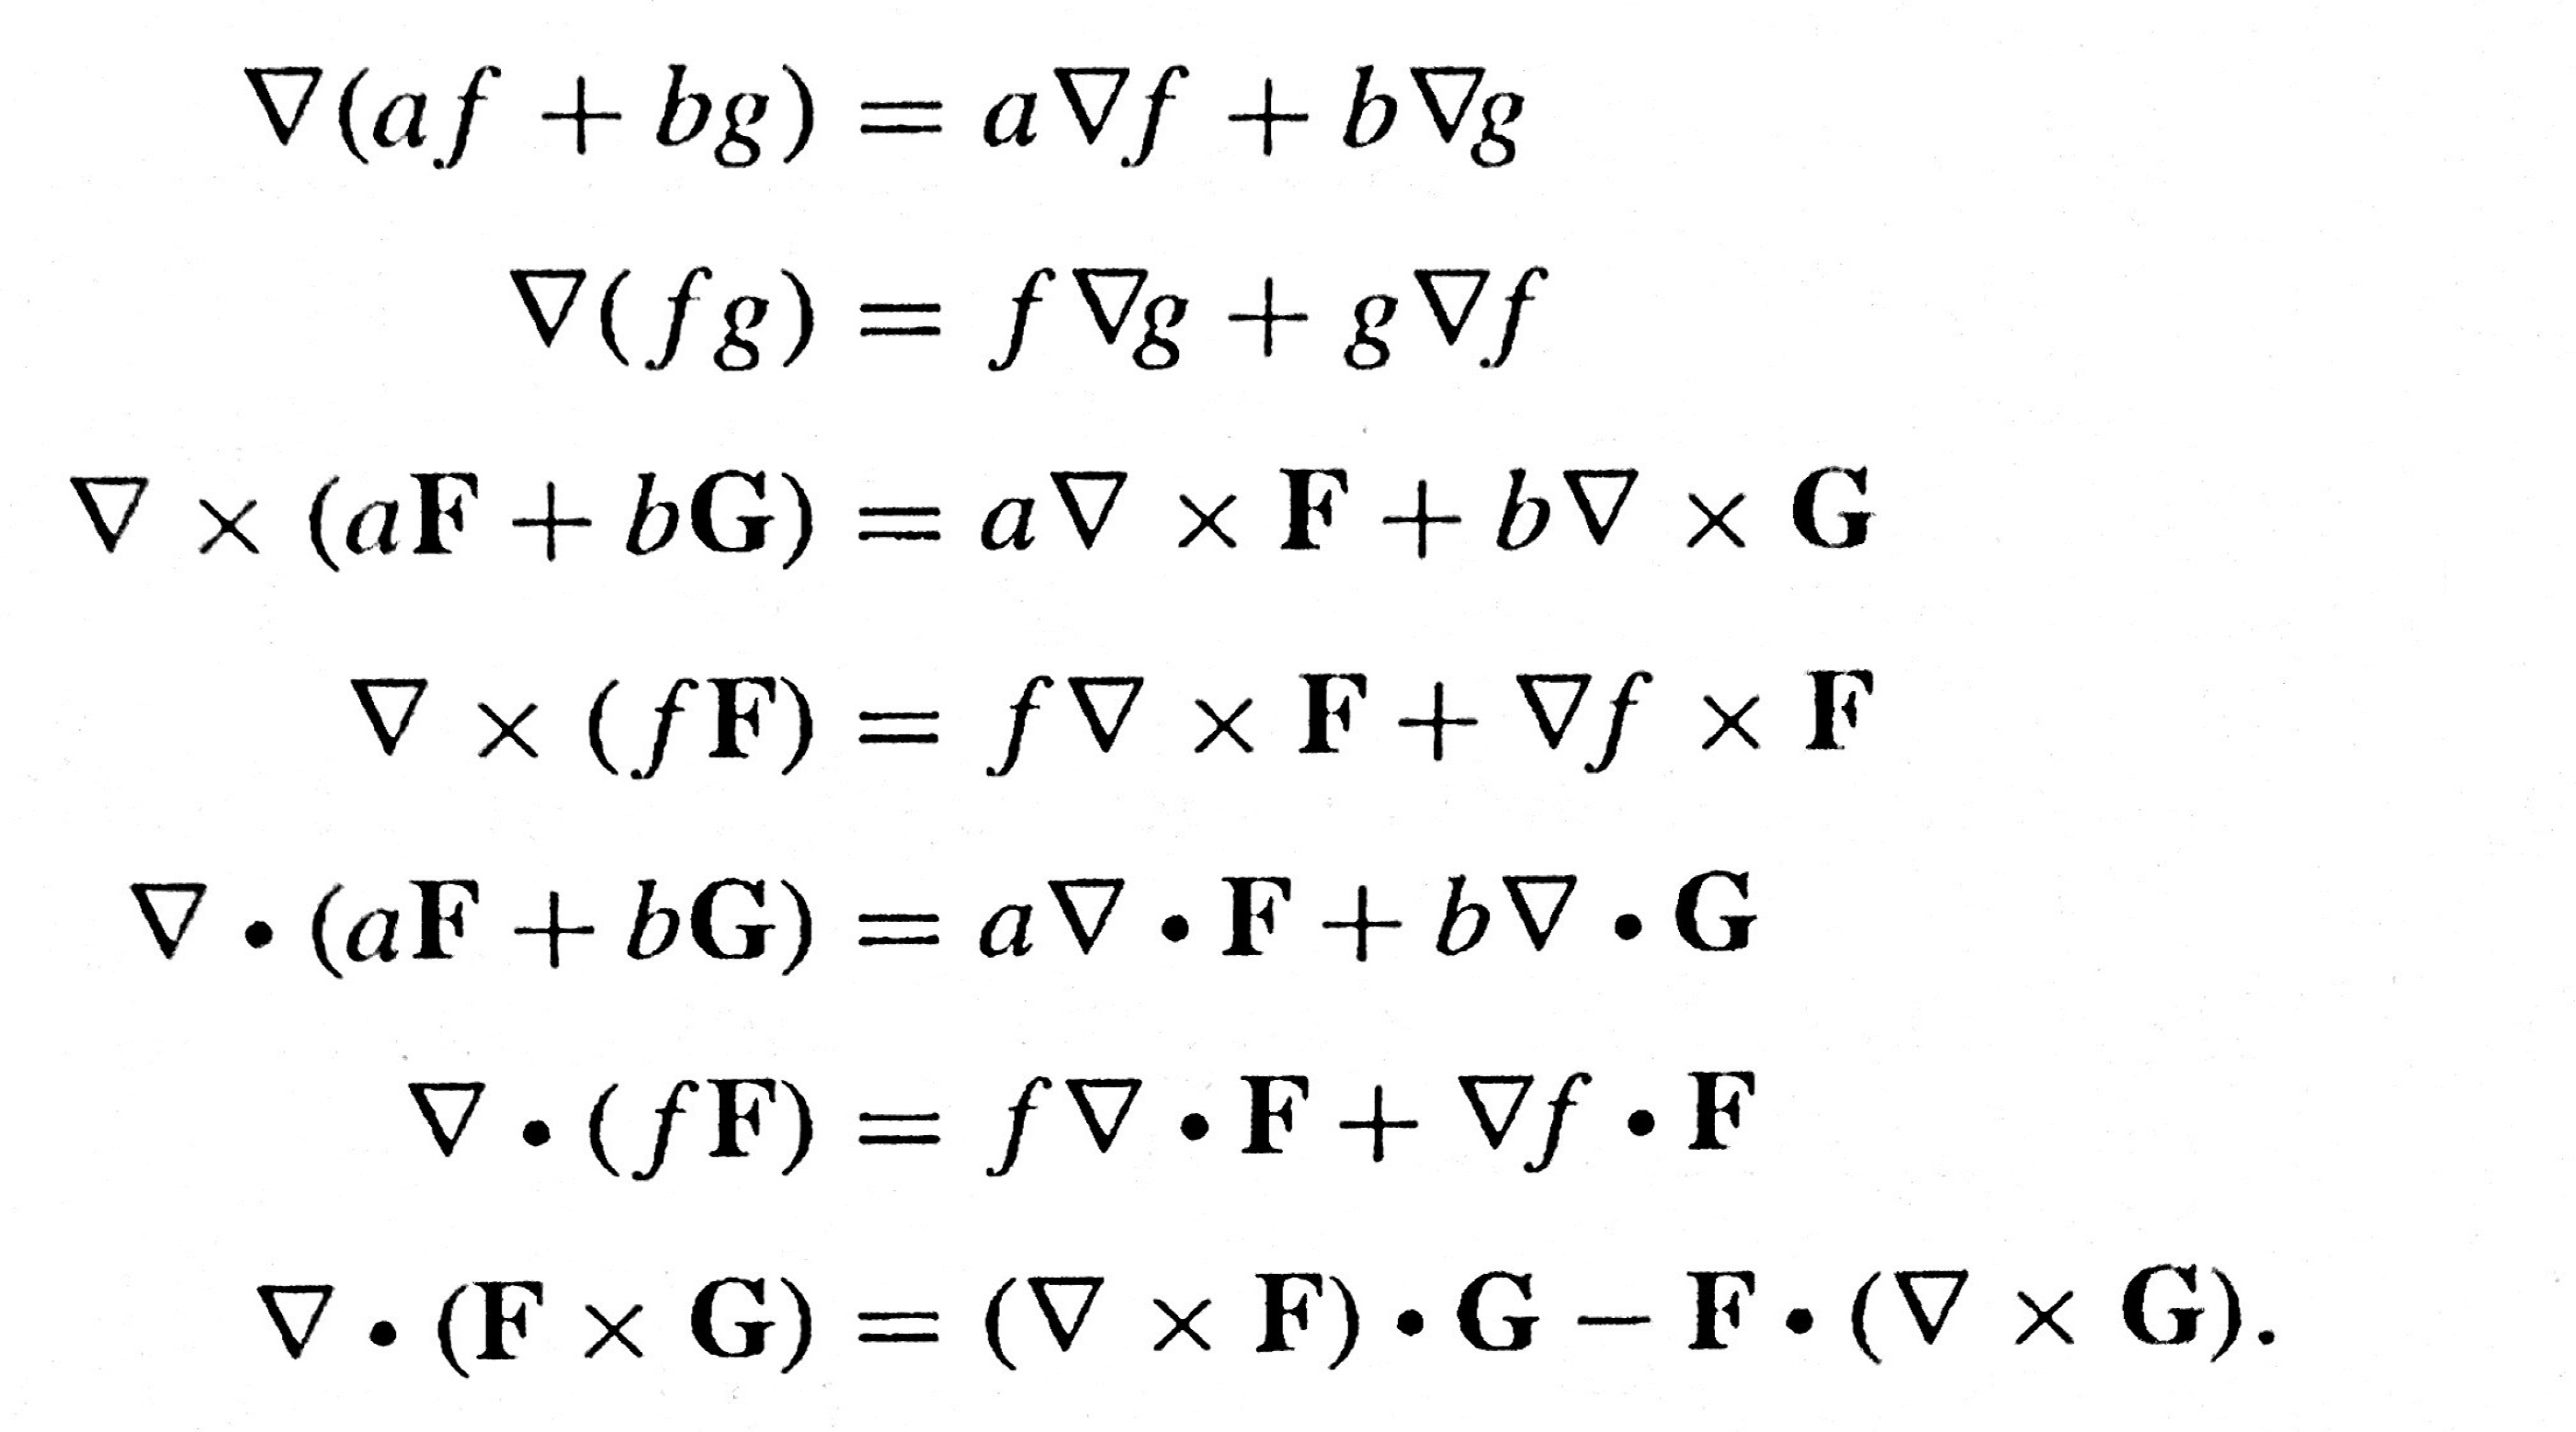
\includegraphics[width=0.8\textwidth]{gradproperties.jpg}
		\caption{Properties of $\nabla$}
		\label{fig:grad}
	\end{figure}
	
	\subparagraph{Green's Identities} If \marginnote{Green's identities?}$\vec{F}$ is assumed to be a gradient field or a multiple $f\nabla g$ of a gradient, then Gauss's formula yields \textbf{Green's first identity}:
		\begin{equation}
			\int_R f\nabla^2 gdV + \int_R \nabla f \cdot \nabla g dV = \int_S f \frac{\partial g}{\partial \vec{n}} d\sigma
		\end{equation}
		From which it is possible to derive \textbf{Green's second identity}:
		\begin{equation}
			\int_R (f\nabla^2 g - g\nabla^2 f)dV = \int_S \left(f \frac{\partial g}{\partial \vec{n}} - g \frac{\partial f}{\partial \vec{n}} \right)d\sigma
		\end{equation}
		
	\subparagraph{Changing Coordinates} If \marginnote{Change of variable and differentials?}$\vec{v}(\vec{x})$ is continuously differentiable and $\vec{x} = T(\vec{u})$ is a coordinate transformation, and $\bar{\mathbf{v}} = \vec{v}(T(\vec{u})$,
		\begin{equation}
			\vec{v}'(\vec{x}) = (\bar{\mathbf{v}} (T^{-1}(\vec{x}))) = \bar{\mathbf{v}}(T^{-1}(\vec{x}))(T^{-1})'(\vec{x})
		\end{equation}
%	\begin{center}
%	\begin{tikzpicture}
%		[scale=3,line cap=round,
%		%Styles
%		axes/.style=,
%		important line/.style={very thick},
%		information text/.style={rounded corners,fill=red!10,inner sep=1ex},
%		dot/.style={circle,inner sep=1pt,fill,label={#1},name=#1}			
%		]
%		
%		%Colors
%		\colorlet{anglecolor}{green!50!black}	%angle arcs/lines
%		
%		%The graphic
%	\end{tikzpicture}
%	\end{center}

%	\begin{figure}[htb]
%		\centering
%		\includegraphics[width=0.8\textwidth]{filename.eps}
%		\caption{Caption.}
%		\label{fig:figure}
%	\end{figure}

%		\def\enotesize{\normalsize}
%		\theendnotes
\end{document}